\PassOptionsToPackage{unicode=true}{hyperref} % options for packages loaded elsewhere
\PassOptionsToPackage{hyphens}{url}
\documentclass[11pt,ignorenonframetext,]{beamer}
\IfFileExists{pgfpages.sty}{\usepackage{pgfpages}}{}
\setbeamertemplate{caption}[numbered]
\setbeamertemplate{caption label separator}{: }
\setbeamercolor{caption name}{fg=normal text.fg}
\beamertemplatenavigationsymbolsempty
\usepackage{lmodern}
\usepackage{amssymb,amsmath}
\usepackage{ifxetex,ifluatex}
\usepackage{fixltx2e} % provides \textsubscript
\ifnum 0\ifxetex 1\fi\ifluatex 1\fi=0 % if pdftex
  \usepackage[T1]{fontenc}
  \usepackage[utf8]{inputenc}
\else % if luatex or xelatex
  \ifxetex
    \usepackage{mathspec}
  \else
    \usepackage{fontspec}
\fi
\defaultfontfeatures{Ligatures=TeX,Scale=MatchLowercase}



  \setmainfont[]{Fira Sans}


  \setmonofont[Mapping=tex-ansi]{Fira Code}


\fi

  \usetheme[]{metropolis}



  \usefonttheme{serif} % use mainfont rather than sansfont for slide text



% use upquote if available, for straight quotes in verbatim environments
\IfFileExists{upquote.sty}{\usepackage{upquote}}{}
% use microtype if available
\IfFileExists{microtype.sty}{%
  \usepackage{microtype}
  \UseMicrotypeSet[protrusion]{basicmath} % disable protrusion for tt fonts
}{}


\newif\ifbibliography


\hypersetup{
      pdftitle={Evaluation Randomisiert-Kontrollierter Studien und Experimente mit },
        pdfauthor={Prof.~Dr.~David Ebert \& Mathias Harrer},
          pdfborder={0 0 0},
    breaklinks=true}
%\urlstyle{same}  % Use monospace font for urls







% Prevent slide breaks in the middle of a paragraph:
\widowpenalties 1 10000
\raggedbottom

  \AtBeginPart{
    \let\insertpartnumber\relax
    \let\partname\relax
    \frame{\partpage}
  }
  \AtBeginSection{
    \ifbibliography
    \else
      \let\insertsectionnumber\relax
      \let\sectionname\relax
      \frame{\sectionpage}
    \fi
  }
  \AtBeginSubsection{
    \let\insertsubsectionnumber\relax
    \let\subsectionname\relax
    \frame{\subsectionpage}
  }



\setlength{\parindent}{0pt}
\setlength{\parskip}{6pt plus 2pt minus 1pt}
\setlength{\emergencystretch}{3em}  % prevent overfull lines
\providecommand{\tightlist}{%
  \setlength{\itemsep}{0pt}\setlength{\parskip}{0pt}}

  \setcounter{secnumdepth}{0}


  \usepackage{calc}
  \usepackage{mathspec}
  \usepackage{booktabs}
  \usepackage{amsmath,amsthm}
  \makeatletter
  \let\@@magyar@captionfix\relax
  \makeatother
  \usepackage{xcolor}
  \usepackage{tikz}
  \definecolor{protectBlue}{RGB}{48,124,148}
  \definecolor{protectGreen}{RGB}{161, 198, 66}
  \definecolor{verywhite}{rgb}{1, 1, 1}
  \usepackage{multicol}
  \hypersetup{colorlinks,citecolor=protectGreen,
    filecolor=red,linkcolor=protectGreen,urlcolor=blue}
  \setbeamercolor{progress bar}{fg=protectGreen}
  \setbeamercolor{alerted text}{fg=protectGreen}
  \setbeamercolor{frametitle}{bg=protectBlue}
  \setbeamercolor{normal text}{fg=protectBlue}
  \titlegraphic{%
  \hspace*{6cm}~%
  
\includegraphics[width=2cm]{assets/logo/tum-lightblue}
  \hspace*{0.3cm}~%
  
\includegraphics[width=2cm]{assets/logo/protect}}
  \setbeamertemplate{frame footer}{Evaluation Randomisiert-Kontrollierter Studien und Experimente mit \textsf{R}}%         <- !!SET FOOTER TITLE!!
  \makeatletter
  \setlength{\metropolis@frametitle@padding}{2.2ex}
  \setbeamertemplate{footline}{%
      \begin{beamercolorbox}[wd=\textwidth, sep=0.7ex]{footline}
          \usebeamerfont{page number in head/foot}%
          \usebeamertemplate*{frame footer}
          \hfill%
          \usebeamertemplate*{frame numbering}
      \end{beamercolorbox}%
  }
  \setbeamertemplate{frametitle}{%
    \nointerlineskip%
    \begin{beamercolorbox}[%
        wd=\paperwidth,%
        sep=0pt,%
        leftskip=\metropolis@frametitle@padding,%
        rightskip=\metropolis@frametitle@padding,%
      ]{frametitle}%
    \metropolis@frametitlestrut@start%
    \insertframetitle%
    \nolinebreak%
    \metropolis@frametitlestrut@end%
    \hfill
    
\includegraphics[height=2ex,keepaspectratio]{assets/logo/tum_white}
    \end{beamercolorbox}%
  }
  \newlength{\cslhangindent}
  \setlength{\cslhangindent}{1.5em}
  \newenvironment{CSLReferences}[3][0]%
  {\setlength{\parindent}{0pt}%
  \everypar{\setlength{\hangindent}{\cslhangindent}}\ignorespaces}%

  \title[]{Evaluation Randomisiert-Kontrollierter Studien und
Experimente mit \textsf{R}}

  \subtitle{Installation von R und RStudio auf dem PC oder MAC}

  \author[
        Prof.~Dr.~David Ebert \& Mathias Harrer
    ]{Prof.~Dr.~David Ebert \& Mathias Harrer}

  \institute[
    ]{
    Psychology \& Digital Mental Health Care, Technische Universität
München
    }

\date[
      Graduiertenseminar TUM-FGZ
  ]{
      Graduiertenseminar TUM-FGZ
        }


\begin{document}

% Hide progress bar and footline on titlepage
  \begin{frame}[plain]
  \titlepage
  \end{frame}



\begin{frame}{Lerninhalte}
\protect\hypertarget{lerninhalte}{}
\textbf{\alert{Block I}} \textbar{} \textbf{R Entdecken} \newline
\checkmark Einführung in R \& RStudio \newline \checkmark R Basics:
Objektklassen, Funktionen, Operatoren, \dots \newline

\textbf{\alert{Block II}} \textbar{} \textbf{Einführung \& Hintergrund}
\newline \checkmark Methodischer Hintergrund von randomisierten Studien
\newline \checkmark Import und Manipulation von Studiendaten mit R
\newline \checkmark Schätzung fehlender Werte \newline

\textbf{\alert{Block III}} \textbar{} \textbf{Analysieren \& Verstehen}
\newline \checkmark Statistische Wirksamkeitsanalyse \newline
\checkmark Alphakorrektur, Effektstärkenberechnung, Visualisierung,
\ldots{}

\begin{tikzpicture}[remember picture,overlay]  
  \node [xshift=4.5cm,yshift=2.5cm] at (current page.center)
    {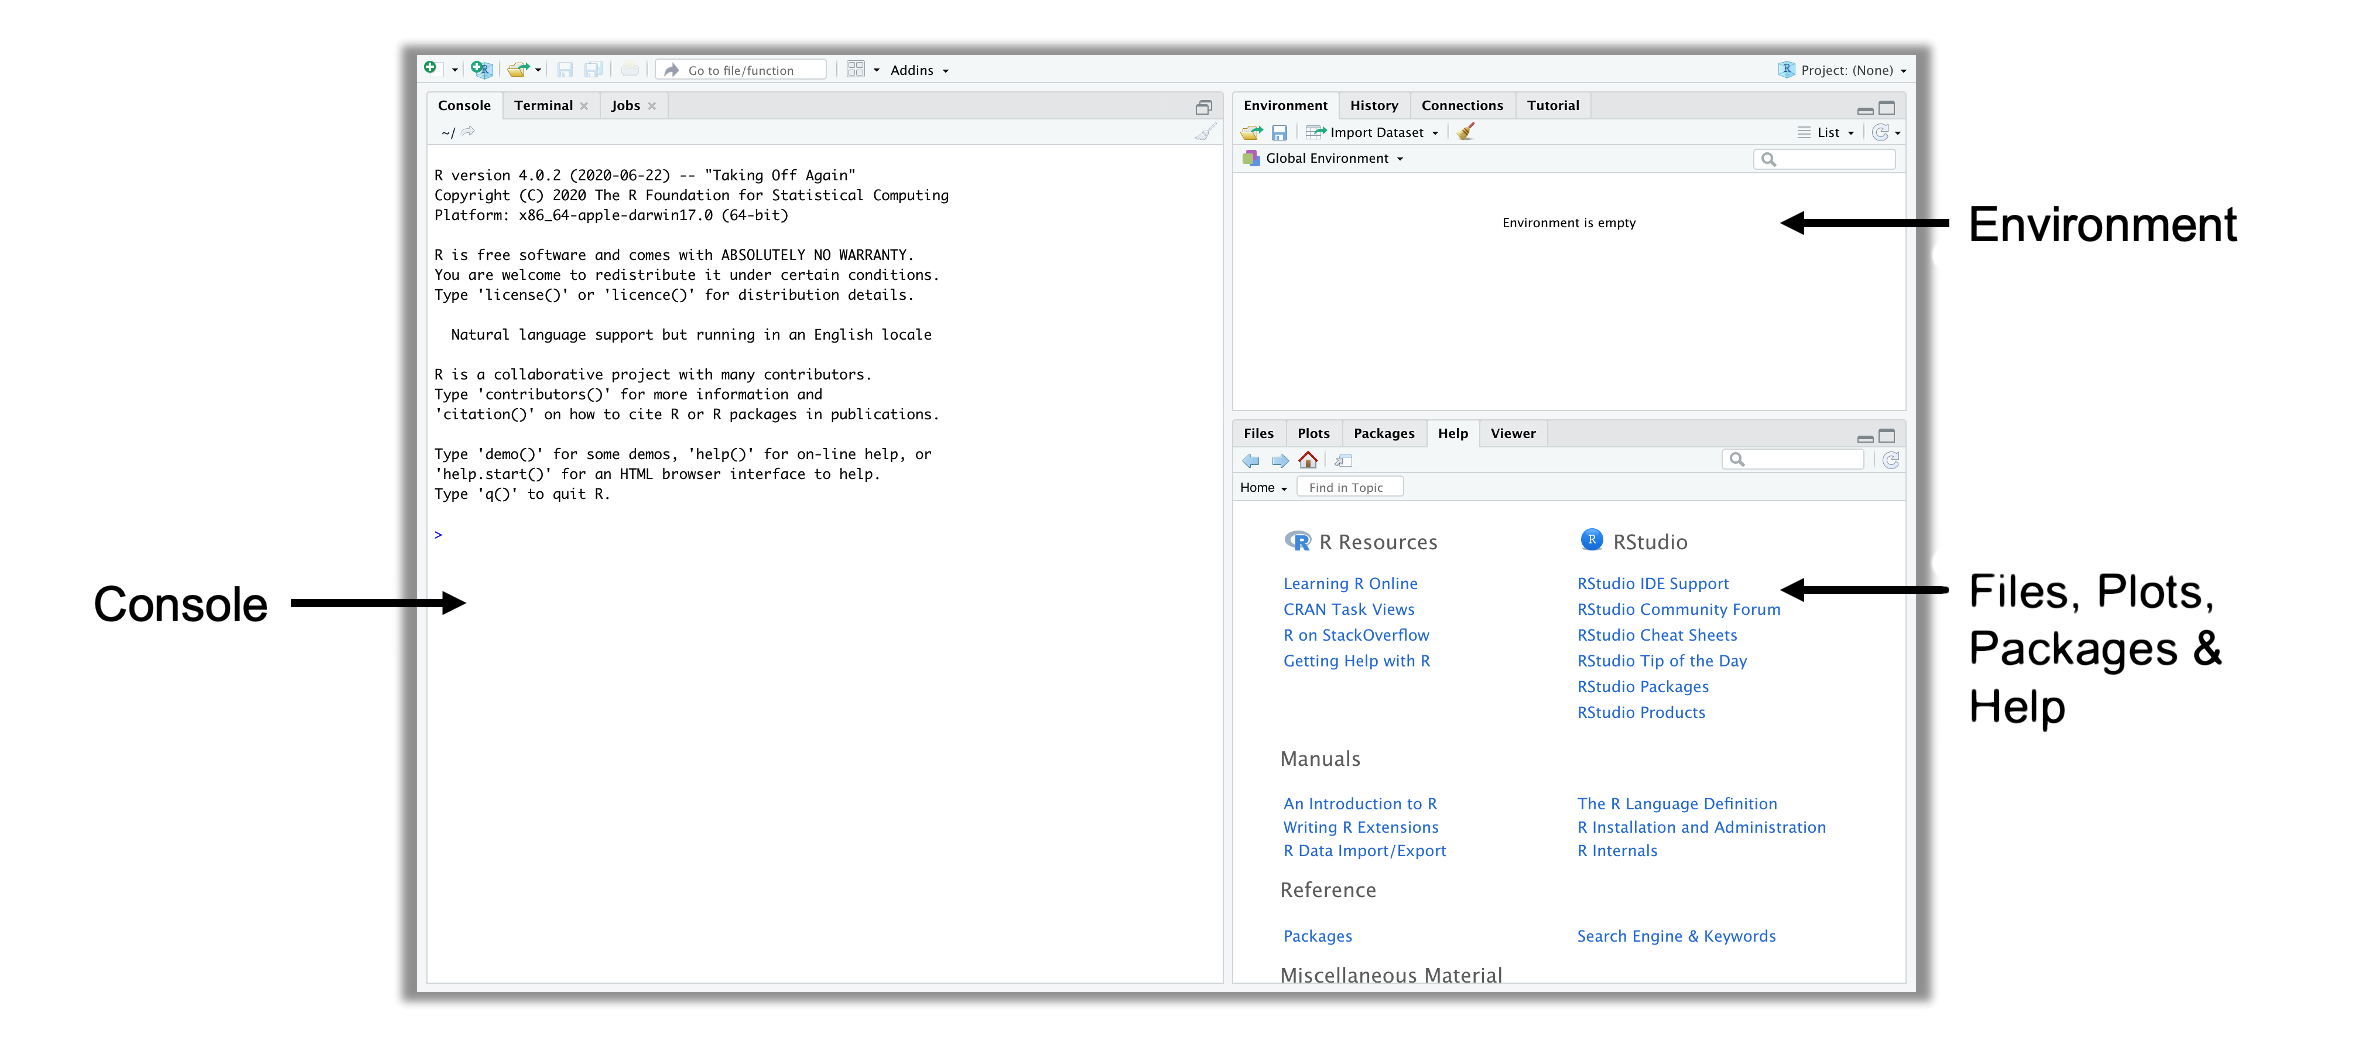
\includegraphics[height=1.5cm]{assets/rs.png}};
\end{tikzpicture}

\begin{tikzpicture}[remember picture,overlay]  
  \node [xshift=4.5cm,yshift=0.2cm] at (current page.center)
    {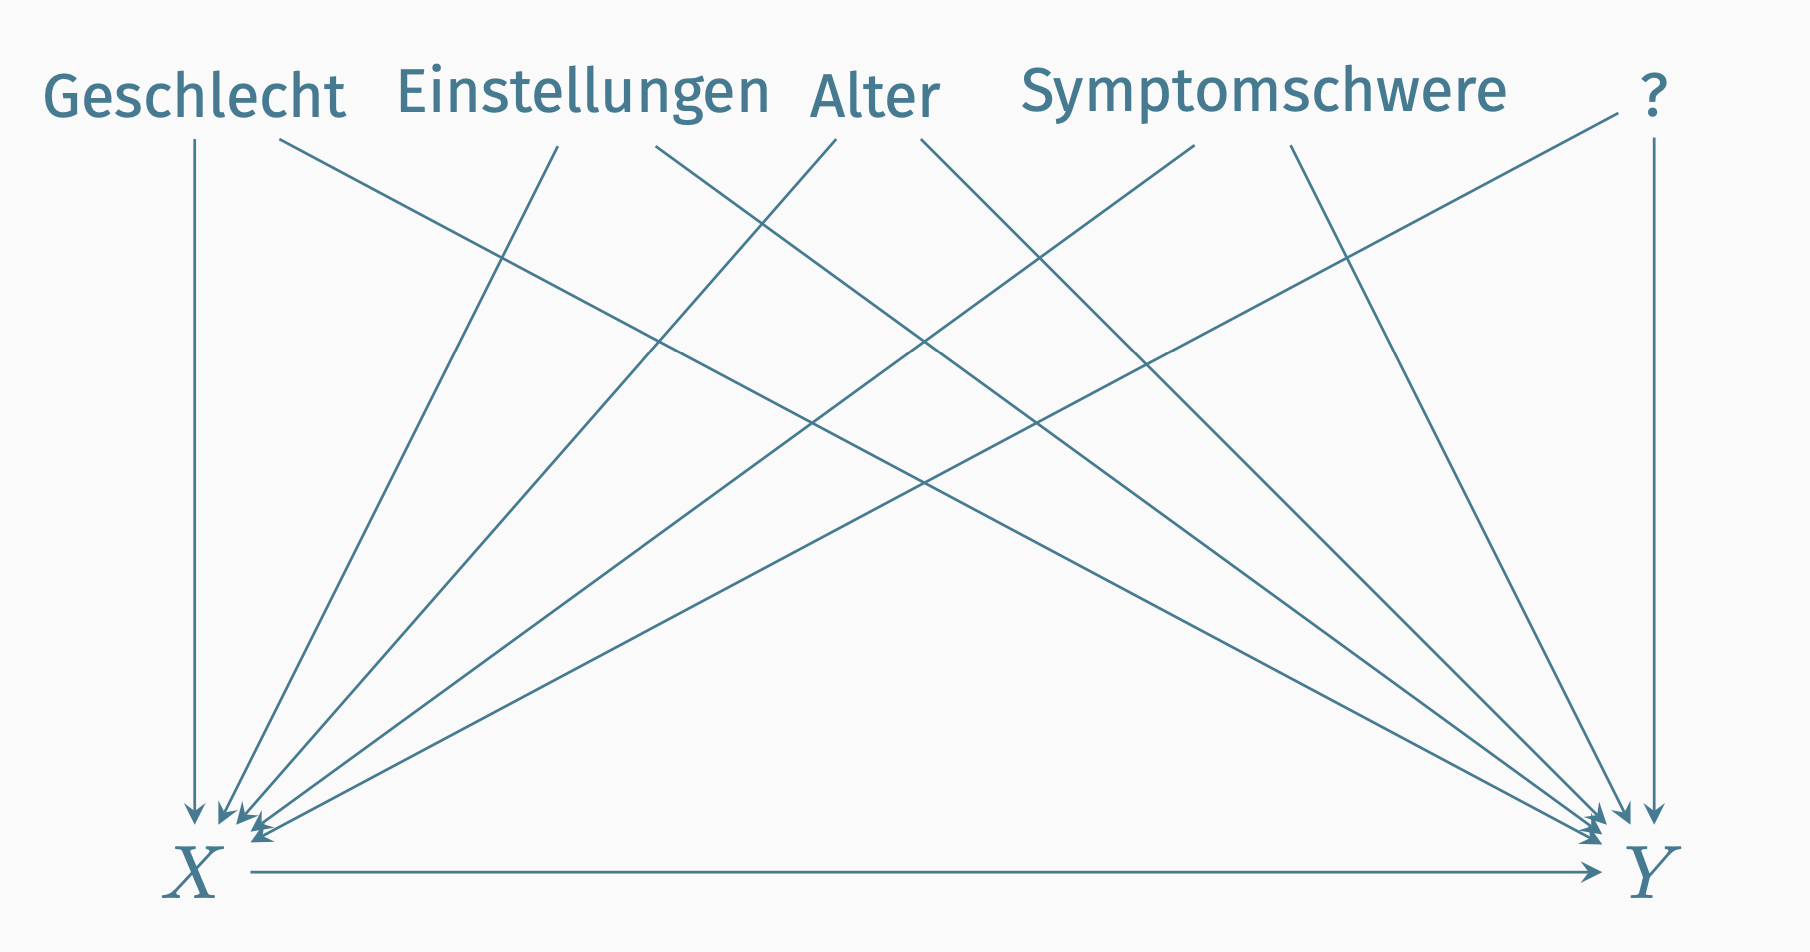
\includegraphics[height=1.5cm]{assets/causal.png}};
\end{tikzpicture}

\begin{tikzpicture}[remember picture,overlay]  
  \node [xshift=4.5cm,yshift=-2cm] at (current page.center)
    {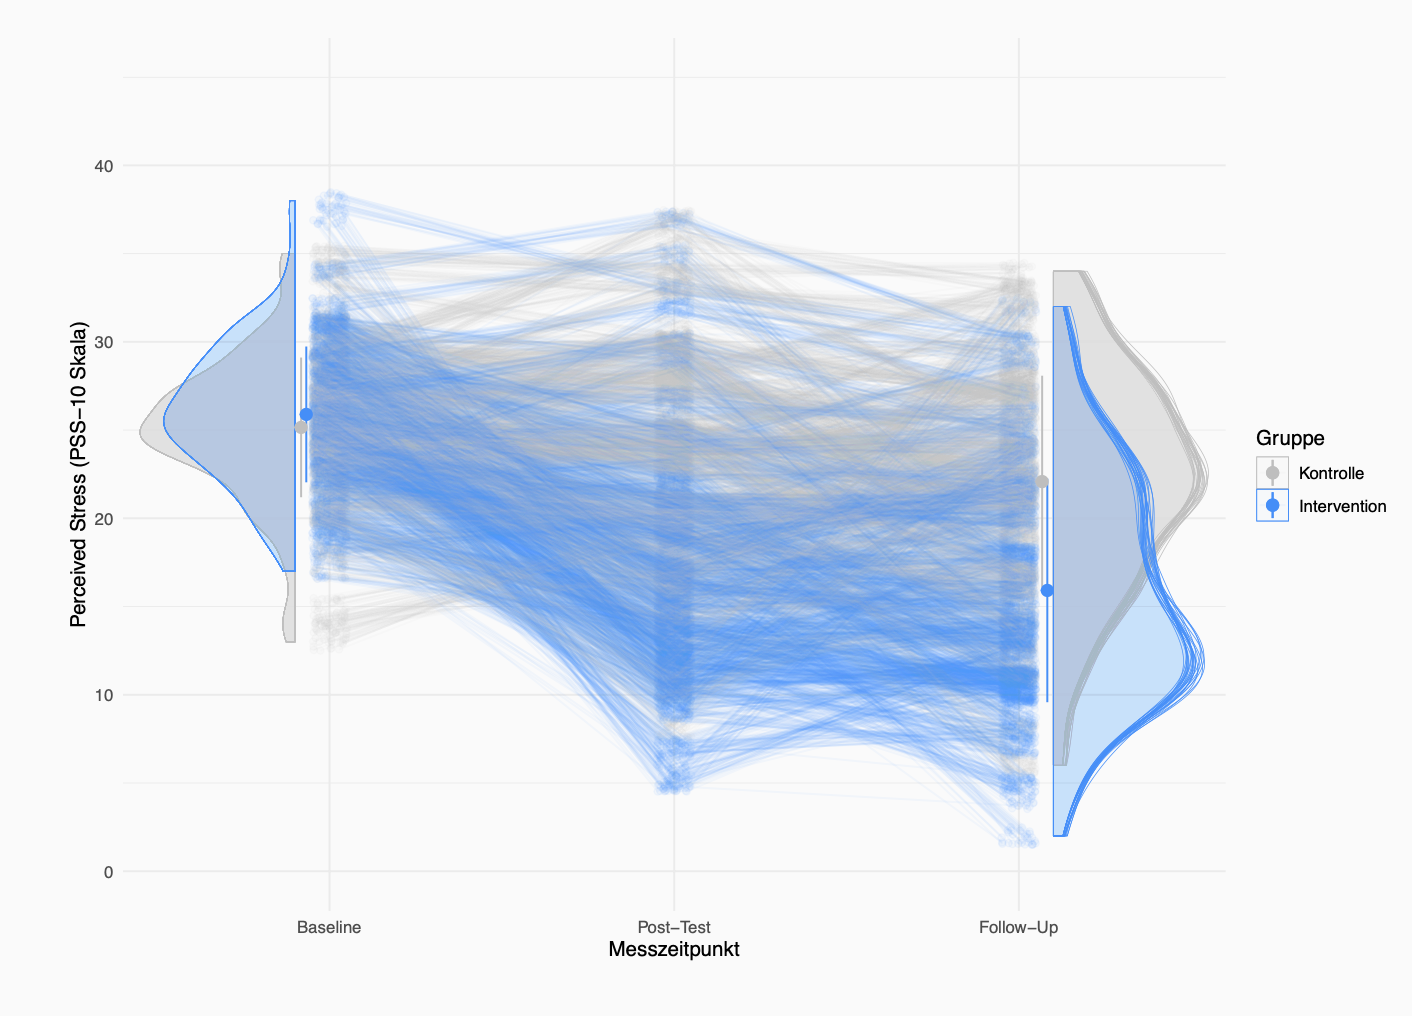
\includegraphics[height=2cm]{assets/raincloud.png}};
\end{tikzpicture}

\begin{tikzpicture}[remember picture,overlay]  
  \node [xshift=0cm,yshift=0cm] at (current page.center)
    {
\includegraphics[width=12cm, height=2.3cm]{assets/opacity.png}};
\end{tikzpicture}

\begin{tikzpicture}[remember picture,overlay]  
  \node [xshift=0cm,yshift=-3cm] at (current page.center)
    {
\includegraphics[width=12cm, height=4cm]{assets/opacity.png}};
\end{tikzpicture}
\end{frame}

\hypertarget{installation-von-r}{%
\section{Installation von R}\label{installation-von-r}}

\begin{frame}{Herunterladen von R}
\protect\hypertarget{herunterladen-von-r}{}
\textbf{R kann von der Comprehensive R Archive Network (CRAN) Website
heruntergeladen werden}

\begin{itemize}
\item
  für Windows:
  \href{https://cran.r-project.org/bin/windows/base/}{cran.r-project.org/bin/windows/base}
\item
  für macOS:
  \href{https://cran.r-project.org/bin/macosx/}{cran.r-project.org/bin/macosx}
\end{itemize}

Eine \textbf{detaillierte Anleitung} zur Installation findet sich z.B.
hier:
\href{http://methods-berlin.com/wp-content/uploads/Installation.html}{Methodengruppe Berlin}.
\end{frame}

\begin{frame}[t]{Versionen von R}
\protect\hypertarget{versionen-von-r}{}
\textbf{Es werden regelmäßig Updates und somit neue Versionen für R zur
Verfügung gestellt}

\metroset{block=fill} 
\begin{exampleblock}{Cave: Veraltete Versionen von R}
  Sollte die Version von \textsf{R} zu veraltet sein, kann es dazu kommen, dass bestimmte Dinge nicht mehr (wie intendiert) funktionieren. R sollte deshalb ca. einmal im Jahr upgedatet werden, indem man die Software neu installiert.
\end{exampleblock}
\end{frame}

\hypertarget{installation-von-rstudio}{%
\section{Installation von RStudio}\label{installation-von-rstudio}}

\begin{frame}{Installation von RStudio}
\metroset{block=fill} 
\begin{block}{Cave: R als Vorbedingung}
  Um RStudio nutzen zu können, muss R bereits vorinstalliert sein.
\end{block}

\textbf{RStudio kann von folgender Website heruntergeladen werden:}

\begin{itemize}
\item
  \href{https://www.rstudio.com/products/rstudio/download/}{rstudio.com/products/rstudio/download}.
\item
  Die \textbf{kostenfreie Version} von RStudio Desktop ist für unsere
  Zwecke ausreichend.
\end{itemize}

Eine \textbf{detaillierte Anleitung} zur Installation findet sich z.B.
wieder hier:
\href{http://methods-berlin.com/wp-content/uploads/Installation.html}{Methodengruppe Berlin}.
\end{frame}




\end{document}
